\documentclass[11pt]{article}
\usepackage[margin=1in]{geometry}
\usepackage[utf8]{inputenc}\usepackage[T1]{fontenc}
\usepackage{hyperref}
\hypersetup{colorlinks=true, linkcolor=blue, citecolor=blue, urlcolor=blue,
  pdftitle={Located, Not Secured}, pdfauthor={Caio Vicentino}}
\emergencystretch=3em \sloppy \hyphenpenalty=2000 \exhyphenpenalty=0 \hbadness=10000
\usepackage{booktabs}\usepackage{amsmath}\usepackage{amssymb}\usepackage{xcolor}\usepackage{array}\usepackage{graphicx}

\title{Located, Not Secured:\\ Principled Limits of Interpretability-Based Control over Agent Actions\\[2pt]
\large A synthesis of one positive lever and five limits, and the turn to auditing}
\author{Caio Vicentino \\ OpenInterpretability \\ Fortaleza, Brazil \\
ORCID: 0009-0003-4331-6259 \\ \texttt{caio@openinterp.org}}
\date{June 2026}

\begin{document}
\maketitle

\begin{abstract}
A recurring hope in agent safety is that mechanistic interpretability will let us \emph{control} an agent:
read an internal state, intervene, and steer behavior. Across an arc of pre-registered studies on an open-weight
reasoning agent (Qwen3.6-27B), we find a sharp and consistent picture. Interpretability \emph{locates} a real,
causal control surface --- a late action-commitment band ($\sim$L51--63) that, unlike the mid-layer ``task-done''
verdict, can elicit and \emph{brake} irreversible actions, generalizing across six actions and three
architectures. But the control it affords is \emph{not securable}, via five limits we make precise: (1)
\textbf{detect $\neq$ control} --- the clean ``done'' feature predicts the stop (AUROC 0.91) yet clamping it does
nothing ($\Delta P = -0.001$); (2) \textbf{felt $\neq$ granted} --- the authorization direction reads the
authorization the model \emph{feels}, allowing 21/21 realistic over-reaches an external check catches; (3)
\textbf{form $\neq$ granted} --- a high-AUROC ``authorization'' direction (0.838) collapses to 0.08 under
structure-matching, i.e. it read scaffold, not concept; (4) \textbf{control $\neq$ robust control} --- the late
brake collapses (attack success $0\to1.0$ at a small budget) under an adaptive white-box adversary; (5)
\textbf{intervention is easy where unneeded} --- in the sincere-error regime a strong reasoning model already
self-corrects, so the intervention is unnecessary, while the regime where it is needed (adversarial) is exactly
where it is fragile. The conclusion: interpretability locates where behavior is decided but does not secure it.
The actionable implication is a regime split --- use interpretability to \emph{audit and monitor} a fixed model
(non-adversarial, where it wins), not to \emph{defend} against an adversary optimizing against a known locus.
\end{abstract}

\section{Introduction}
If an agent is about to do something harmful and we can \emph{see} it internally, can we \emph{stop} it? The
appeal of interpretability-based control --- refusal directions, representation rerouting, feature clamping,
activation steering --- rests on a yes. This paper synthesizes a pre-registered arc that answers: interpretability
\emph{locates} the control surface, and sometimes acts through it, but the control is not securable. We state one
positive result and five principled limits, each from a separate study with the same causal-rigor protocol
(random-feature baseline, control-token normalization, structural-rigidity sweep, structure-matched control,
behavioral confirmation). The synthesis is not a counsel of despair: it is a redirection. Where interpretability
\emph{loses} (adversarial control) is not where it is most useful; where it \emph{wins} (non-adversarial auditing)
is, and a companion result---\emph{The Late Channel}~\cite{latechannel}---shows what that looks like.

\section{Interpretability locates the control surface (the positive)}
For a long-horizon coding agent, control of the termination decision lives not at the mid-layer ``task is done''
verdict but in a late action-commitment block ($\sim$30 layers downstream, L51--63): a task-matched late donor
flips a real \texttt{finish} (42\%, $p{=}0.031$) while the verdict layer is inert~\cite{leverlate}. This late lever
\emph{generalizes} --- finish$\to$edit, and from eliciting to \emph{braking} --- and works as a brake on genuinely
irreversible actions: a simulated \texttt{send\_transaction} collapses $0.998\to0.00$ with 100\% redirect to a safe
action, replicating across six action domains and three architectures~\cite{levergen,brake}. A single late-layer
``authorization direction'' both detects \emph{and} controls an agent's commitment to unauthorized irreversible
actions~\cite{authdir}. \textbf{Interpretability locates a real, causal, generalizing control surface.} The rest
of the paper is about what that surface does \emph{not} give us.

\section{Limit 1 --- Detect $\neq$ control}
The ``task complete / all tests pass'' feature is clean, interpretable, and predicts the \texttt{finish} action
(AUROC 0.91). Yet clamping it to its success value at the decision point yields $\Delta P(\texttt{finish}) =
-0.001$ ($p{=}0.44$) --- identical to a random feature~\cite{verdict}. The model \emph{represents} ``done'' as a
named feature, but that is not what makes it stop. Detection is not control, even at the exact, named feature.

\section{Limit 2 --- Felt $\neq$ granted (blind to a class of error)}
On a real filesystem agent, the authorization probe is operationally blind to the realistic model-origin error:
it allows 21/21 over-reaches the agent makes in good faith (CI $[0.845,1.0]$), while an external, task-grounded
check catches all 21~\cite{felt}. The probe reads the authorization the model \emph{feels}, not the one the user
\emph{granted}. An internal monitor inherits the model's own judgment error --- so defense-in-depth is necessary,
because the internal and external failure modes are disjoint.

\section{Limit 3 --- Form $\neq$ granted (confoundable)}
A frozen ``authorization'' direction with AUROC 0.838 collapses to 0.08 under structure-matching: it had separated
on conversation structure, lexicon, and punctuation, not the concept~\cite{form}. A high cross-context AUROC
without a named, structure-controlled feature is not evidence of a concept --- a lesson that became a mandatory
naming + structure-matched gate in the protocol.

\section{Limit 4 --- Control $\neq$ robust control}
The same late action-commitment brake that suppresses \texttt{send\_transaction} ($1.00\to0.00$) is reopened by an
adaptive white-box adversary that knows the brake layer and donor: a budget-4 signed-Adam embedding-space attack
takes attack success $0\to1.0$, while a norm-matched random perturbation does nothing (companion result, this
arc). The locus that \emph{controls} in the benign regime is not adversarially robust --- mirroring the broader
finding that representation- and detection-level defenses fall to adaptive attacks.

\section{Limit 5 --- Intervention is easy where unneeded}
Finally, even granting a working detector, the act it triggers is caught in a bind. On 32 agent-trap scenarios,
the strong reasoning model already chose the safe action without any chain-of-thought in 30/32 cases --- in the
\emph{sincere-error} regime it self-corrects, so an intervention is unnecessary. The regime where intervention is
needed is the adversarial one (Limit 4), where mechanical injection collapses and a behavioral re-prompt can be
rationalized. Reliable action exists where it is least needed; where the error is real, no intervention is robust.

\section{Synthesis: locating is not securing}
\begin{figure}[h]\centering
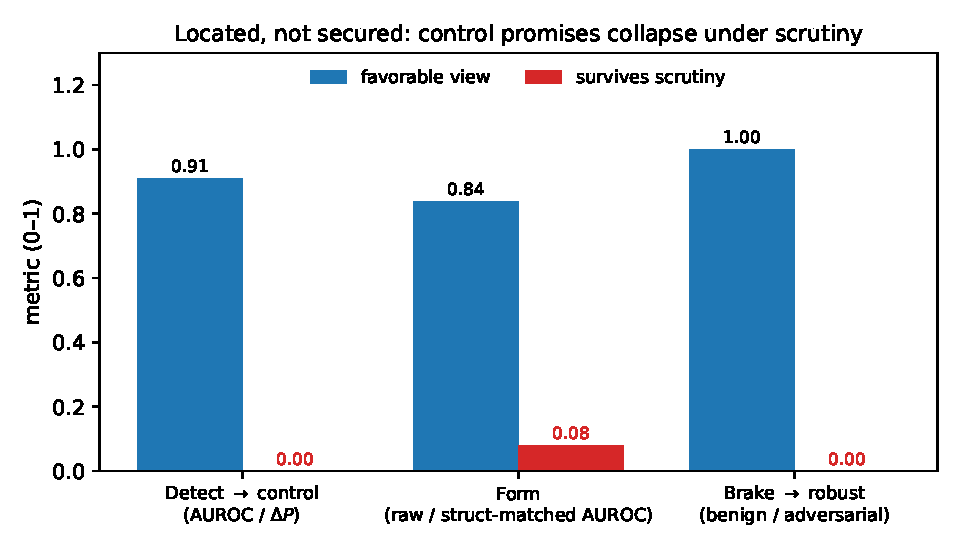
\includegraphics[width=0.74\textwidth]{fig_located.pdf}
\caption{Three of the five limits, as matched pairs with identical semantics --- a favorable interpretability
metric (blue) vs what survives the right control (red): detection AUROC 0.91 vs control effect $\approx 0$; raw
AUROC 0.838 vs structure-matched 0.08; benign brake suppression vs adversarial robustness ($1-\text{ASR}$). The
other two limits (felt $\neq$ granted, intervention easy where unneeded) concern an internal monitor's blind spot
and are qualitative --- stated in the text and Table~\ref{tab:syn}, not plotted.}\label{fig:located}
\end{figure}
\begin{table}[h]\centering\small
\begin{tabular}{lll}
\toprule
 & What interpretability gives & The limit \\
\midrule
Locate the lever & late action band, causal, generalizes & --- (this part works) \\
Detect the state & ``done'' feature, AUROC 0.91 & clamping does nothing ($\Delta P\!=\!-0.001$) \\
Read authorization & a late direction & reads \emph{felt}, allows 21/21 real over-reaches \\
Trust the AUROC & 0.838 separability & 0.08 under structure-matching \\
Brake the action & $1.0\to0.0$ suppression & $0\to1.0$ under adaptive attack \\
Act on the trigger & inject or re-prompt & easy where unneeded, fragile where needed \\
\bottomrule
\end{tabular}
\caption{One positive lever, five limits. Control power rises toward the late action channel; security guarantees
do not follow it.}\label{tab:syn}
\end{table}
Locating \emph{where} behavior is decided is necessary but nowhere near sufficient for \emph{securing} it. The
limits are orthogonal: error-blindness, confoundability, non-robustness, and the easy-where-unneeded bind are
different holes, none closed by a better localization.

\section{Implication: a regime split}
Why does interpretability-based control lose here? The adversarial-control regime lets an optimizer move
activations against a known locus; activation malleability then makes it a losing game by construction. But the
same internal access \emph{wins} in the non-adversarial \emph{auditing} regime --- a fixed model examined as a
scientific object, with no optimizer fighting the probe. ``Detect $\neq$ control'' stops mattering when the goal
is detect/understand, not control-under-attack. The companion result \emph{The Late Channel}~\cite{latechannel}
shows this concretely: the same late band that fails as a robust control point is a readable, causal locus for
\emph{monitoring} a reasoning agent. The recommendation that falls out of the whole arc: use interpretability to
audit and monitor, not to defend.

\section{Methods (the through-line)}
Every result above passed one causal-rigor protocol: random-feature and shuffled-label baselines, control-token
normalization for steering, a structural-rigidity $\alpha$-sweep, a structure-matched control and feature naming,
behavioral confirmation (a real generation, not a logit), and paired exact tests. This shared discipline is what
lets five separate negatives be read as one principled picture rather than a string of failures.

\section{Limitations}
Simulated decision points; white-box interventions; a single model family (with two cross-architecture checks);
modest $n$ in several studies; the adversarial attacks use a strong continuous-embedding threat model whose
deployment realism is contested. The positive (the located lever) is the smallest-$n$ result; the load-bearing
claims here are the limits, which are robust.

\begin{thebibliography}{99}\small
\bibitem{leverlate} Vicentino. The Lever Is Late. 2026. Zenodo 10.5281/zenodo.20534219.
\bibitem{levergen} Vicentino. The Lever Generalizes --- and It Brakes. 2026. Zenodo 10.5281/zenodo.20672840.
\bibitem{brake} Vicentino. Mechanistic Circuit-Breakers Generalize Across Irreversible Agent Actions and Architectures. 2026. Zenodo 10.5281/zenodo.20679287.
\bibitem{authdir} Vicentino. The Authorization Direction. 2026. Zenodo 10.5281/zenodo.20683623.
\bibitem{verdict} Vicentino. The Verdict Is Not the Lever. 2026. Zenodo 10.5281/zenodo.20532769.
\bibitem{felt} Vicentino. Felt, Not Granted. 2026. Zenodo 10.5281/zenodo.20685264.
\bibitem{form} Vicentino. Form, Not Granted. 2026. Zenodo 10.5281/zenodo.20724650.
\bibitem{latechannel} Vicentino. The Late Channel. 2026. Zenodo 10.5281/zenodo.20752896.
\end{thebibliography}
\end{document}
